Rendszerünk öt fő komponensből áll, amelyeket a komponens diagramon is láthatunk: egy Ruby on Rails keretrendszerben írt API-ból, egy Vue.js alapú webes felhasználói- és admin felületből, egy Flutter alkalmazásból a felhasználók számára, valamint egy Flutter keretrendszerben készült POS terminál alkalmazásból. Az API a REST architektúrát követi, lehetővé téve a különböző erőforrások, például buszok, járatok és jegyek kezelését. A felhasználói és admin weboldal Vue-ban készült, a Vuetify elemek felhasználásával, ami lehetővé tette az egyszerű és hatékony felhasználói felületek gyors fejlesztését. A Vue.js keretrendszer előnye, hogy komponensekből áll, így átlátható és jól rendszerezett webalkalmazás felépítést tesz lehetővé. Ezen kívül a Vuetify komponens-készlete megkönnyítette az UI elemek létrehozását, gyorsítva ezzel a fejlesztési folyamatot. Az alkalmazás Flutterben készült, Dart programozási nyelvet használva, amely lehetővé teszi, hogy ugyanazt a kódbázist használjuk iOS és Android platformokra is, így jelentősen csökkentve a fejlesztési időt és költségeket. A POS terminál alkalmazása is Flutter keretrendszerben készült, biztosítva a hatékony és egységes megoldást a különböző platformok számára.
A Vue.js alapú weboldalakat, illetve a felhasználóknak szánt Flutter alkalmazást Portik Szabolcs kollegám mutatja be részletesebben egy másik dolgozat 
keretein belül.

\begin{figure}[H]
    \centering
    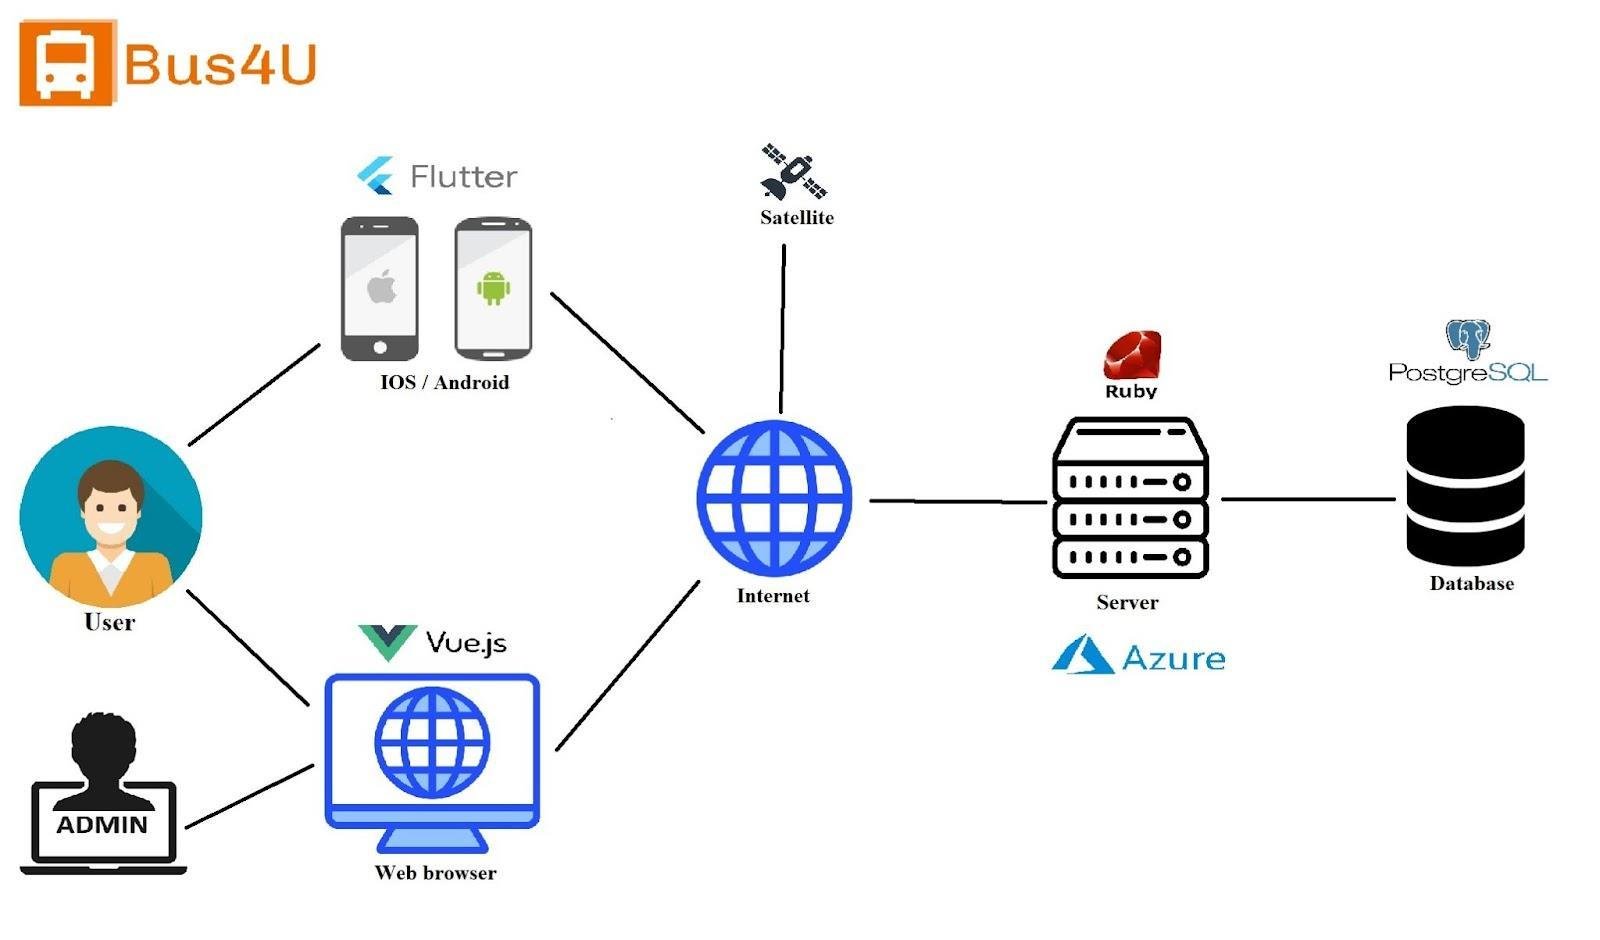
\includegraphics[width=\textwidth]{figures/component.jpg}
    \caption{A rendszer komponensdiagramja}
    \label{fig:component-diagram}
  \end{figure}


\section{Az API felépítése}
A Bus4U API a REST architektúrát követi, és számos végpontot biztosít a különböző erőforrások kezeléséhez, mint például:
\begin{itemize}
    \item \textbf{Buszok kezelése}: buszok létrehozása, frissítése, törlése.
    \item \textbf{Járatok menedzselése}: járatok lekérése és ütemezése.
    \item \textbf{Jegyek és bérletek}: jegyek és bérletek vásárlása és kezelése.
\end{itemize}

\section{Endpointok részletes leírása}

\subsection{GET /get\_stations\_by\_city}
Ez az endpoint lehetővé teszi a megállók listájának lekérését egy adott város alapján. A kérés a következő paramétert használja:
\begin{itemize}
    \item \textbf{city\_uid}: A város egyedi azonosítója.
\end{itemize}

\textbf{Példa kérés}:
\begin{verbatim}
GET https://api.bus4u.online/v1/get_stations_by_city?city_uid=CTY_N11XH
\end{verbatim}

\textbf{Válasz formátum}:
\begin{verbatim}
{
    "stations": [
        {
            "station_uid": "STT_EGAVX",
            "name": "Sapientia",
            "address": "Str. Calea Sighisoarei nr. 2",
            "longitude": "24.59883",
            "latitude": "46.52339"
        },
        {
            "station_uid": "STT_6CO3Q",
            "name": "Dedeman",
            "address": "Bul. 1 Decembrie nr. 189",
            "longitude": "24.59941",
            "latitude": "46.52678"
        }
    ]
}
\end{verbatim}

\section{Adatkezelés és adatbázis kapcsolat}
Az API végpontjai a \textbf{PostgreSQL} adatbázissal kommunikálnak. Az adatbázis tranzakciókat az \textbf{ActiveRecord} ORM segítségével kezeljük, amely lehetővé teszi az adatok egyszerű és hatékony lekérését, beszúrását és frissítését.

\subsection{Adatbázis táblák}
A PostgreSQL adatbázisunk a következő táblákból áll:
\begin{itemize}
    \item \textbf{Companies}: Azon cégek adatai, akikkel szerződést kötött a Bus4U.
    \item \textbf{Admins}: Különböző cégekhez tartozó adminisztrátorok adatai. Szerepük lehet “boss” vagy “driver”.
    \item \textbf{Buses}: A cégekhez tartozó autóbuszok adatai.
    \item \textbf{Routes}: A cégek saját útvonalai.
    \item \textbf{Stations}: A rendszerben található buszmegállók összessége.
    \item \textbf{Route\_stations}: Egy cég adott útvonalán keresztülhaladó megállók.
    \item \textbf{Timetables}: Egy útvonal megállójának indulási időpontjai és ára nap szerinti felosztásban.
    \item \textbf{Cities}: Az összes város, amelyen áthaladnak útvonalak.
    \item \textbf{Users}: A Bus4U felhasználói a fontosabb adataikkal.
    \item \textbf{Email\_verifications}: Az adott email címekhez tartozó regisztrációkor felhasználandó kódok.
    \item \textbf{Tickets}: A felhasználókhoz tartozó jegyek.
    \item \textbf{Payments}: Stripe fizetések eltárolása.
\end{itemize}

\begin{figure}[H]
    \centering
    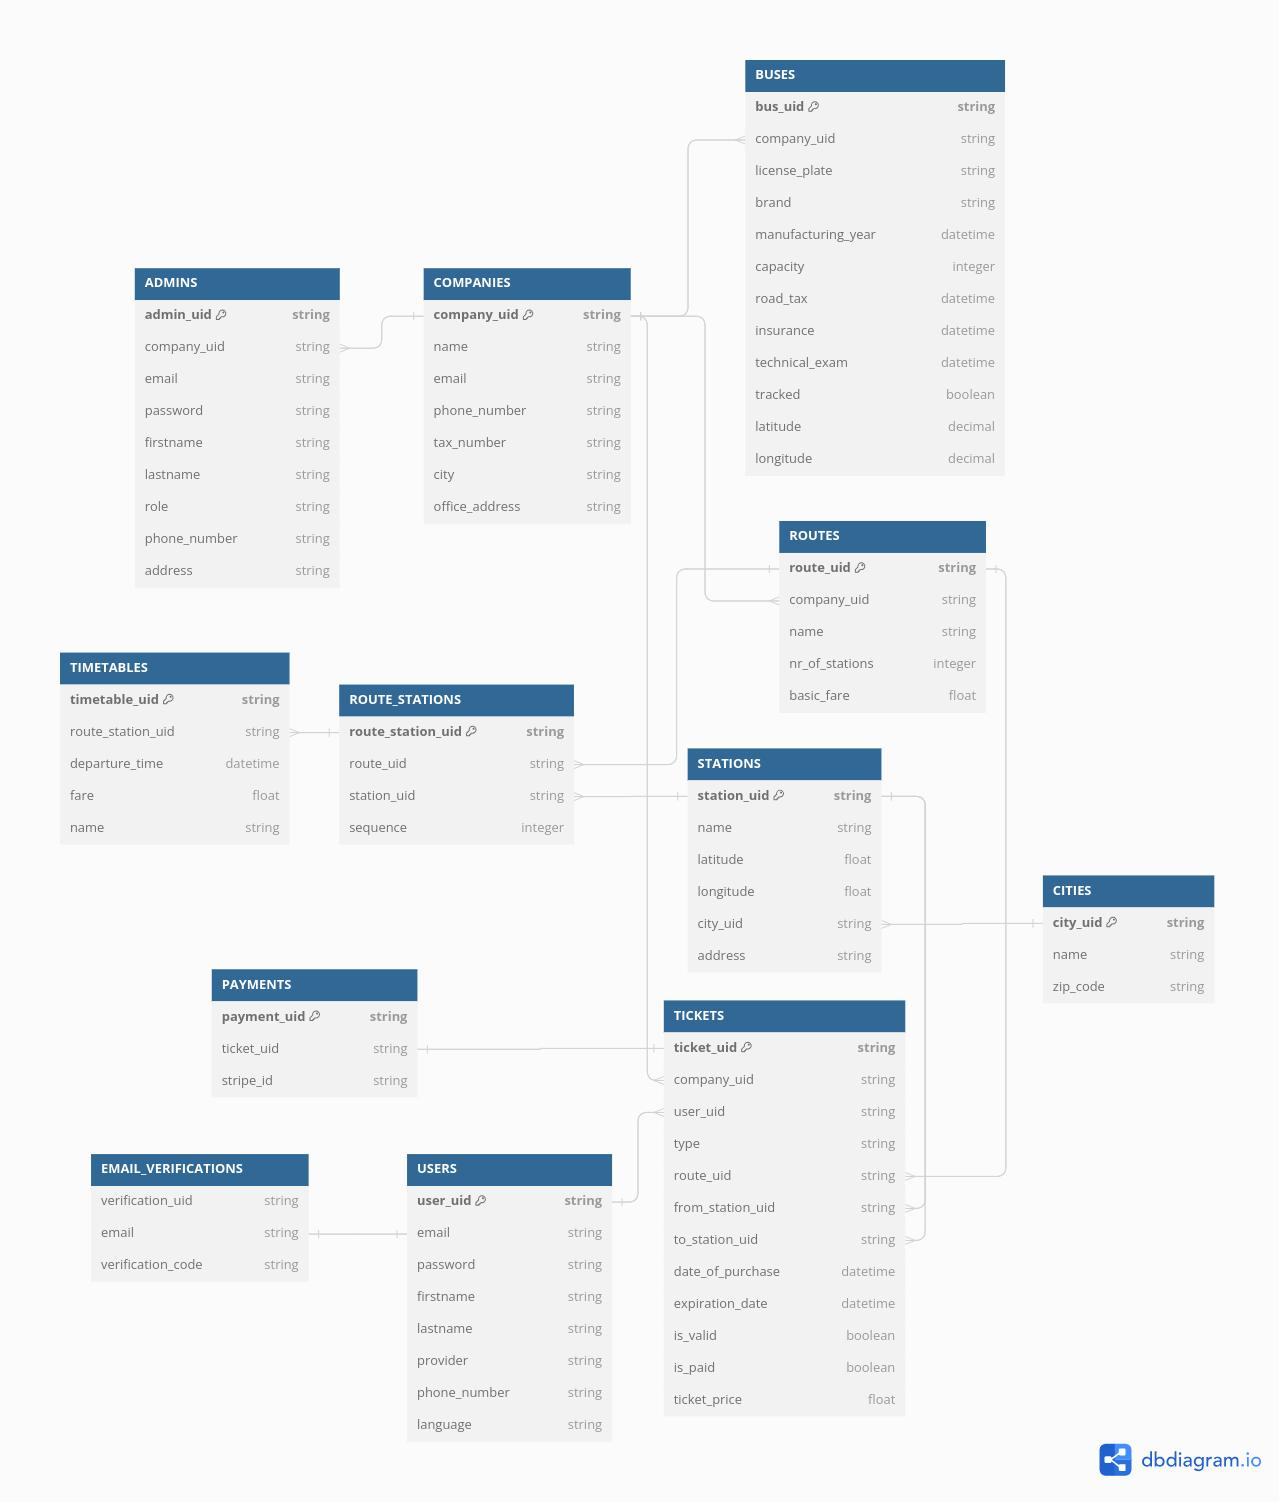
\includegraphics[width=\textwidth]{figures/database.jpg}
    \caption{Az rendszer adatbázisdiagramja}
    \label{fig:database-diagram}
  \end{figure}

  \section{Projektmenedzsment és verziókövetés}

  A projekt fejlesztése során több eszközt alkalmaztunk a feladatok nyomon követésére, a fejlesztési folyamat szervezésére és a forráskód verziókövetésére.
  
  \subsection{Jira}

  A projektmenedzsment során a \textbf{Jira} kanban boardját használtuk, amely az Atlassian által fejlesztett projekt-követő platform. A Jirát választottuk, mert egy olyan hatékony eszköz, amely egyszerre letisztult, ám funkciókban komplex, így könnyedén igazítható a projekt igényeihez. 
  
  A Kanban tábla három fő oszlopból állt:
  \begin{itemize}
      \item \textbf{To do}: Ide kerültek azok a feladatok, amelyeket még nem kezdtünk el.
      \item \textbf{In progress}: Ebben az oszlopban azok a feladatok szerepeltek, amelyek éppen folyamatban voltak.
      \item \textbf{Done}: Az elvégzett feladatok ebbe az oszlopba kerültek, jelezve azok befejezését.
  \end{itemize}
  
  Minden feladatot hozzárendeltünk egy konkrét tulajdonoshoz, valamint címkékkel láttunk el, amelyek megjelölték, hogy a munka épp a rendszer melyik komponensére vonatkozik: \textbf{API}, \textbf{felhasználói felület}, \textbf{admin felület}, vagy \textbf{mobil alkalmazás}. A feladatok ilyen címkézése segített abban, hogy pontosan tudjuk, ki mivel foglalkozik, illetve milyen állapotban van a fejlesztés különböző területein végzett munka.

  \begin{figure}[H]
    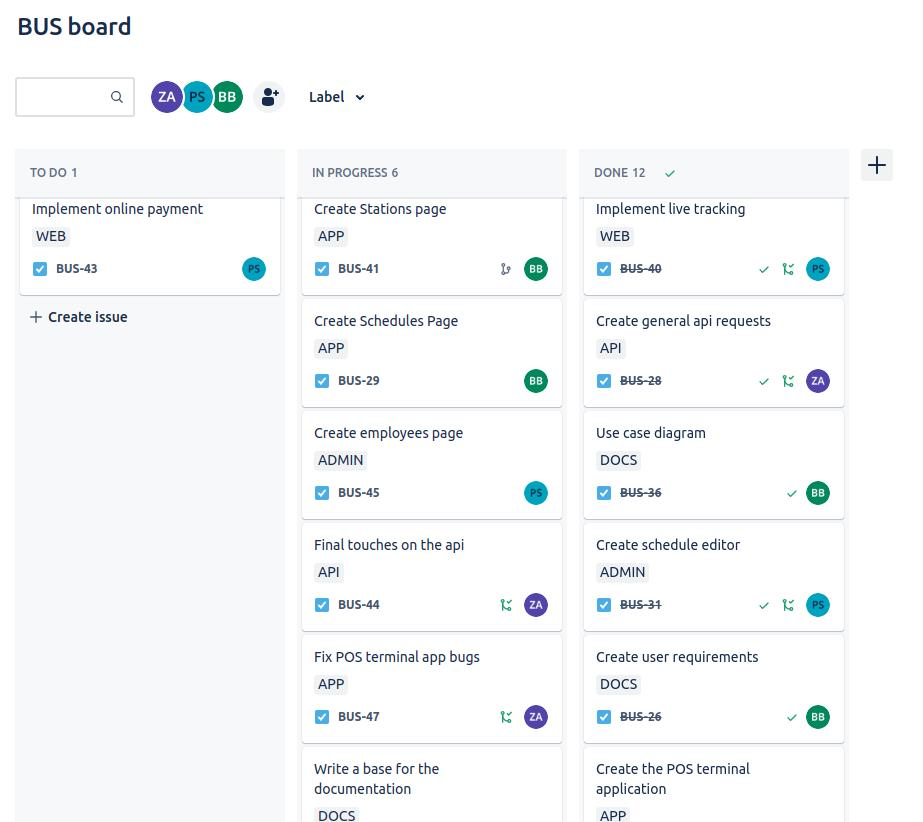
\includegraphics[width=\textwidth]{figures/jira.jpg}
    \caption{A Jira kanban board áttekintése}
    \label{fig:jira}
  \end{figure}
      
  \subsection{Git és GitHub}

  A projekt forráskódjának verziókezelését a \textbf{Git} verziókezelő rendszer segítségével oldottuk meg, míg a kód tárolására a \textbf{GitHub} platformot használtuk. A GitHub lehetőséget biztosított a pull request-ek hatékony kezelésére, amelyekkel minden változtatást egyszerűen tudtunk jóváhagyni. Ez a megközelítés a kód visszakövethetőségét és dokumentálását is jelentősen megkönnyítette, hozzájárulva a kód minőségének javításához és a fejlesztési folyamat átláthatóságához.
  
  A projekt struktúráját három fő \textbf{branch} köré szerveztük:
  \begin{itemize}
      \item \textbf{main branch}: Ebbe az ágba kizárólag a már teljesen tesztelt és stabil kódrészletek kerültek be, amelyeket időszakosan publikáltunk. Ez az ág szolgált a hivatalos, működőképes verzió tárolására.
      \item \textbf{develop branch}: A develop branch-et a fejlesztés és tesztelés helyszíneként használtuk. Az ide feltöltött kódok még tesztelés alatt álltak, de a fejlesztési idő alatt mindig a develop verzióját futtattuk az Azure környezetben, ezzel biztosítva, hogy az aktuális fejlesztések folyamatosan elérhetők és tesztelhetők legyenek.
      \item \textbf{feature branchek}: Az új funkciók fejlesztését különálló, ún. feature branchekben végeztük, amelyek a konkrét feladatokra vagy kódrészletekre koncentráltak. Például kisebb munkaigényű kódok, mint az általános API lekérések fejlesztése külön branchekben történt, míg az összetettebb funkciókat külön feature branch-ekben dolgoztuk ki.
  \end{itemize}
  
  A branch-ek ilyen felosztása lehetővé tette a párhuzamos fejlesztést, és biztosította, hogy a különböző fejlesztési szakaszok kódjai elkülönítve és rendezetten legyenek tárolva. A GitHub pull request funkciójának köszönhetően minden változtatást felül tudtunk vizsgálni, így minden módosítás előtt biztosak lehettünk annak minőségében és kompatibilitásában.

  \begin{figure}[H]
    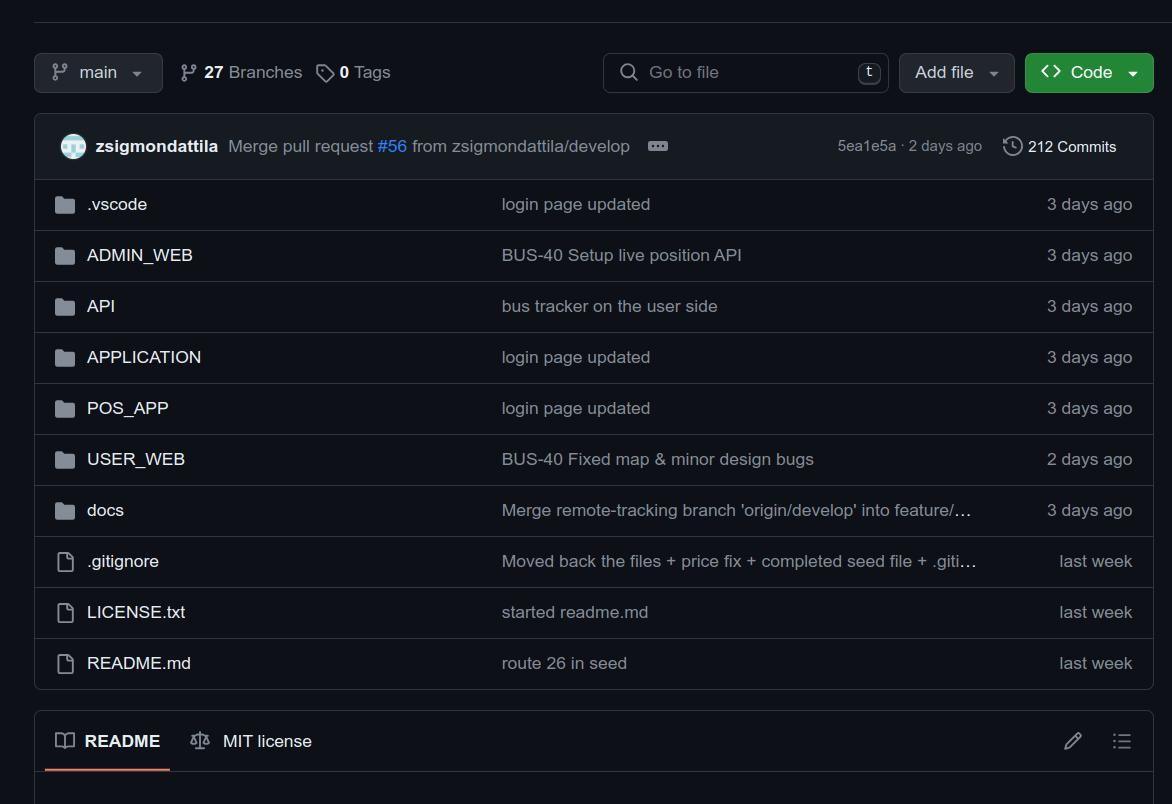
\includegraphics[width=\textwidth]{figures/github.jpg}
    \caption{A GitHub repository áttekintése}
    \label{fig:github}
  \end{figure}
  
  
  Ezek az eszközök hozzájárultak a projekt sikeres és hatékony fejlesztéséhez, elősegítve a feladatok egyértelműsítését, priorizálását és a csapat tagjai közötti együttműködést.
  
